\section{Resultate}
In diesem Kapitel werden die Ergebnisse der durchgeführten Untersuchung vorgestellt und analysiert.

\subsection{Ergebnisse des Modelltrainings} \label{chap:ergebnisse-modelltraining}
Beim Modelltraining wurden keine Erfolge mit den VGG- und AlexNet-Modellen erzielt, da diese Modelle nach dem Training alles als positiv klassifizieren. Der ViT erzielte ebenfalls schlechte Ergebnisse beim COVIDx-Datensatz, konnte jedoch den MRI-Datensatz im Vergleich besser erlernen.

\begin{figure}[ht!]
    \centering
    \begin{subfigure}{0.5\linewidth}
        \centering
        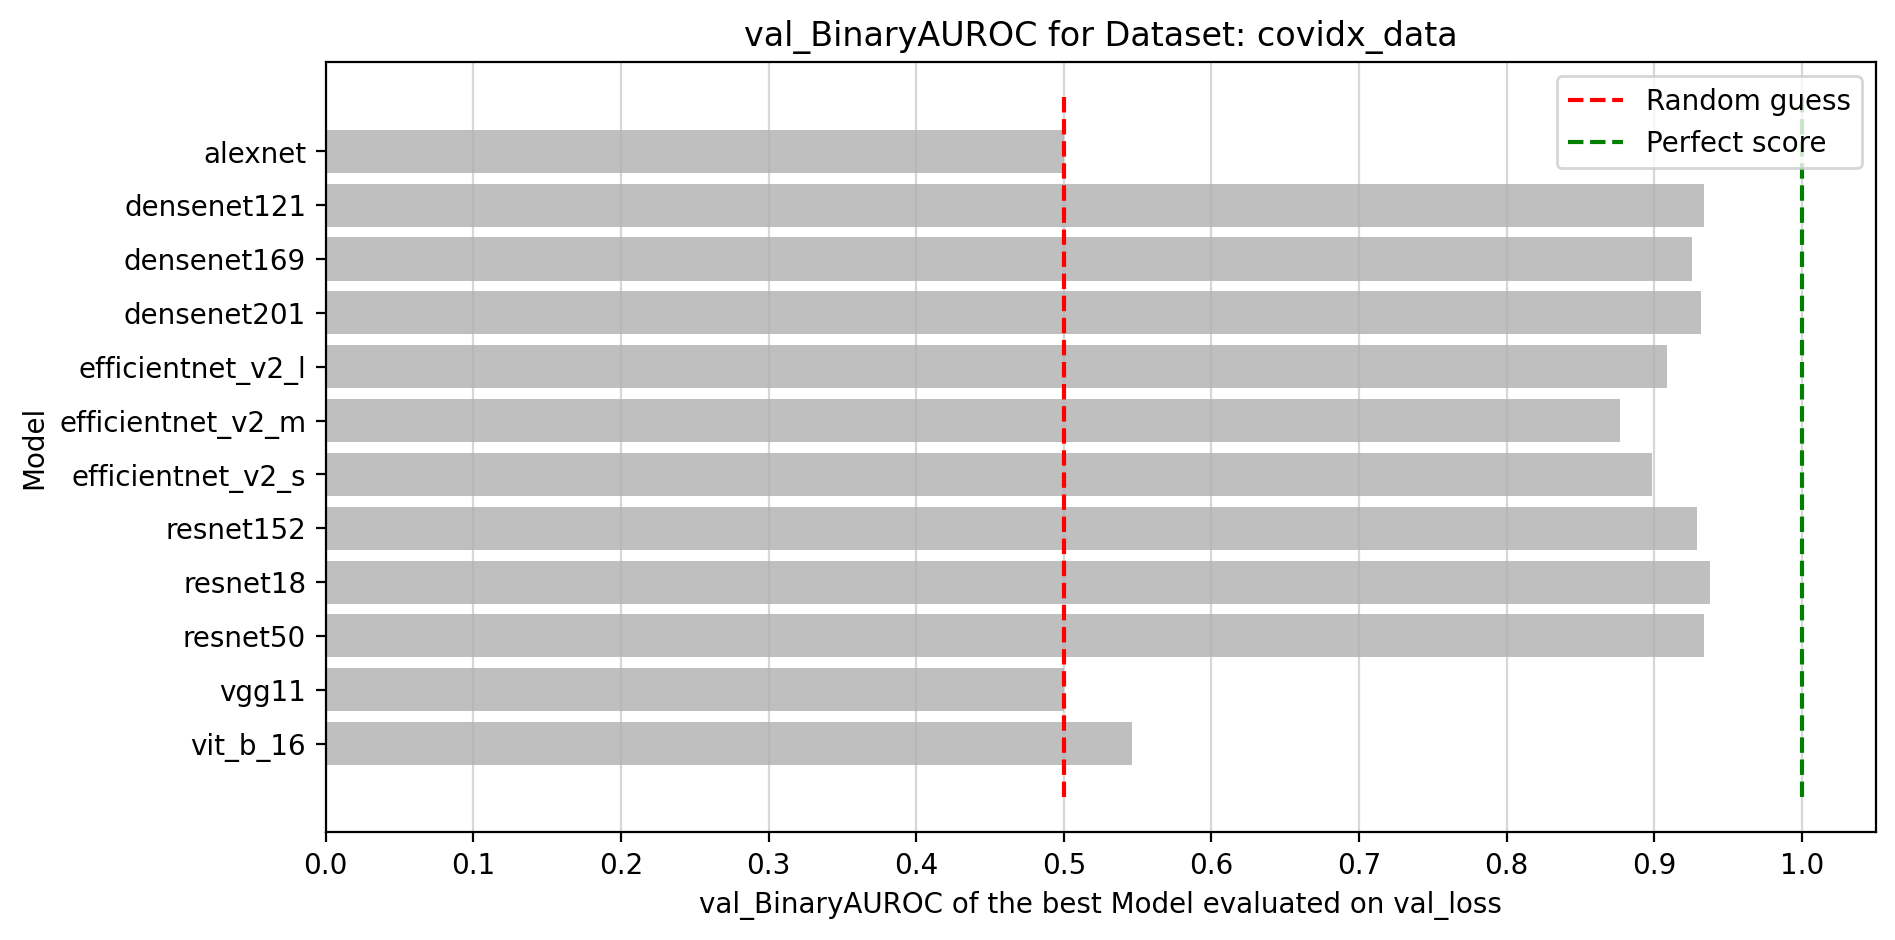
\includegraphics[height=0.5\linewidth]{01-images/05-resultate/val_binaryAUROC_COVIDX.png}
        \caption{AUROC-Validierungsmetrik für den COVIDx-Datensatz}
    \end{subfigure}\hfill%
    \begin{subfigure}{0.5\linewidth}
        \centering
        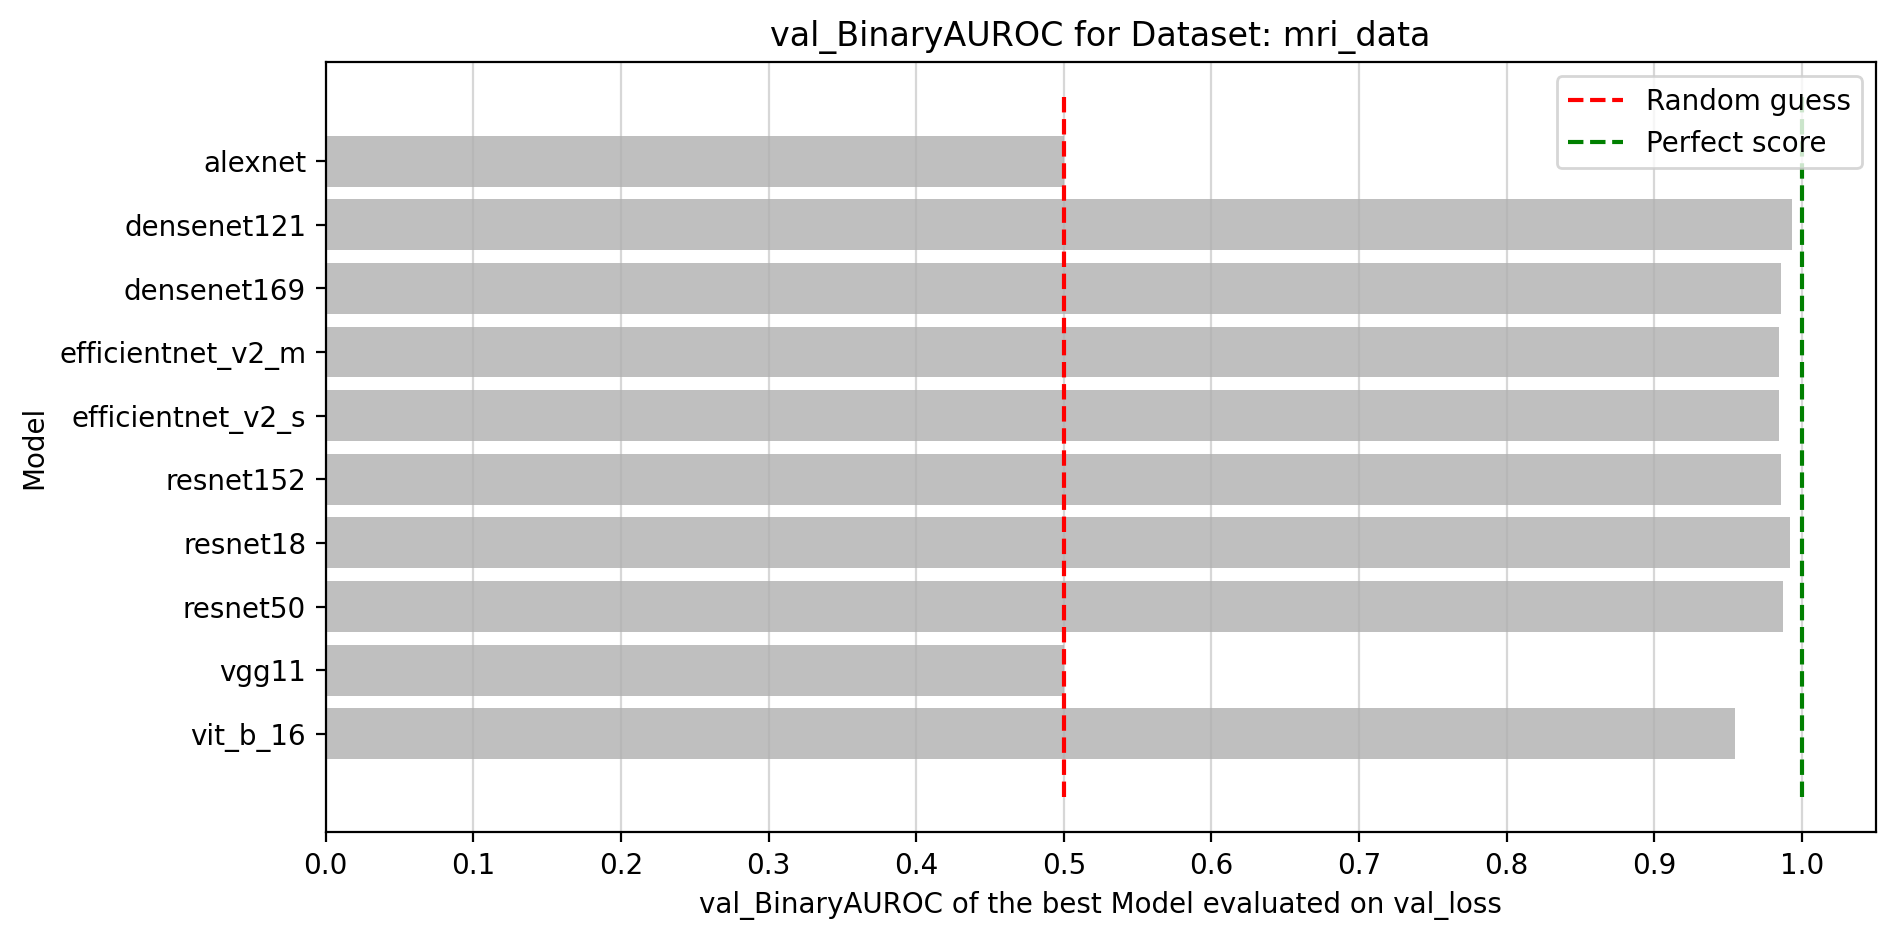
\includegraphics[height=0.5\linewidth]{01-images/05-resultate/val_binaryAUROC_MRI.png}
        \caption{AUROC-Validierungsmetrik für den MRI-Datensatz}
    \end{subfigure}
    \caption{Die AUROC-Validierungsmetriken der besten Modelle im Trainingslauf, gemessen an der val\_loss-Metrik}
\end{figure}

Beim Vergleich der oberen und der unteren Grafiken zeigt sich eine klare Differenz zwischen den AUROC Validierungs- und Testmetriken auf den Datensätzen, wobei die Modelle auf den Validierungsdaten zu overfitten scheinen, obwohl beim Training nur die Lernrate optimiert wurde und das beste Modell anhand des Validierungslosses ausgewählt wurde. Beim Training der Modelle wurden keine weiteren Regularisierungen eingesetzt. Die Differenz der Metriken könnte durch mögliche Unterschiede in den Verteilungen der Partitionen, wie in den Kapiteln \ref{chap:COVID19-datenverteilung} und \ref{chap:brain-datenverteilung} diskutiert, erklärt werden. 

\begin{figure}[ht!]
    \centering
    \begin{subfigure}{0.5\linewidth}
        \centering
        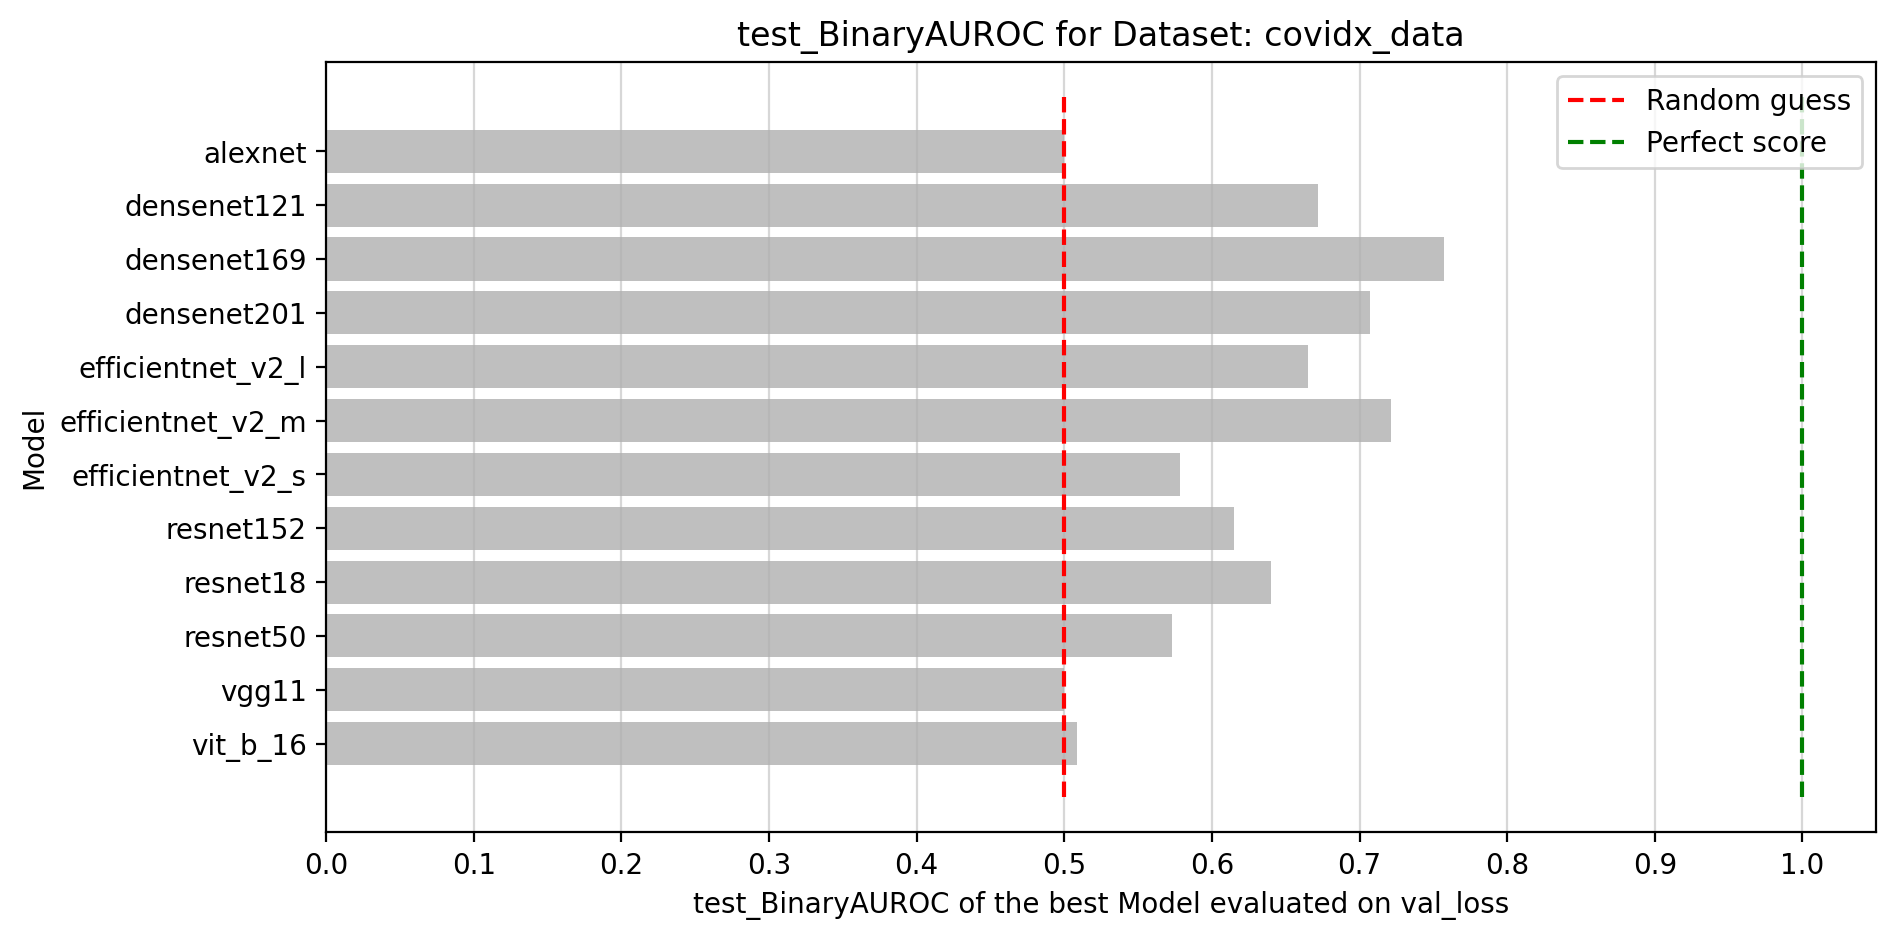
\includegraphics[height=0.5\linewidth]{01-images/05-resultate/test_binaryAUROC_COVIDX.png}
        \caption{AUROC-Testmetrik für den COVIDx-Datensatz}
    \end{subfigure}\hfill%
    \begin{subfigure}{0.5\linewidth}
        \centering
        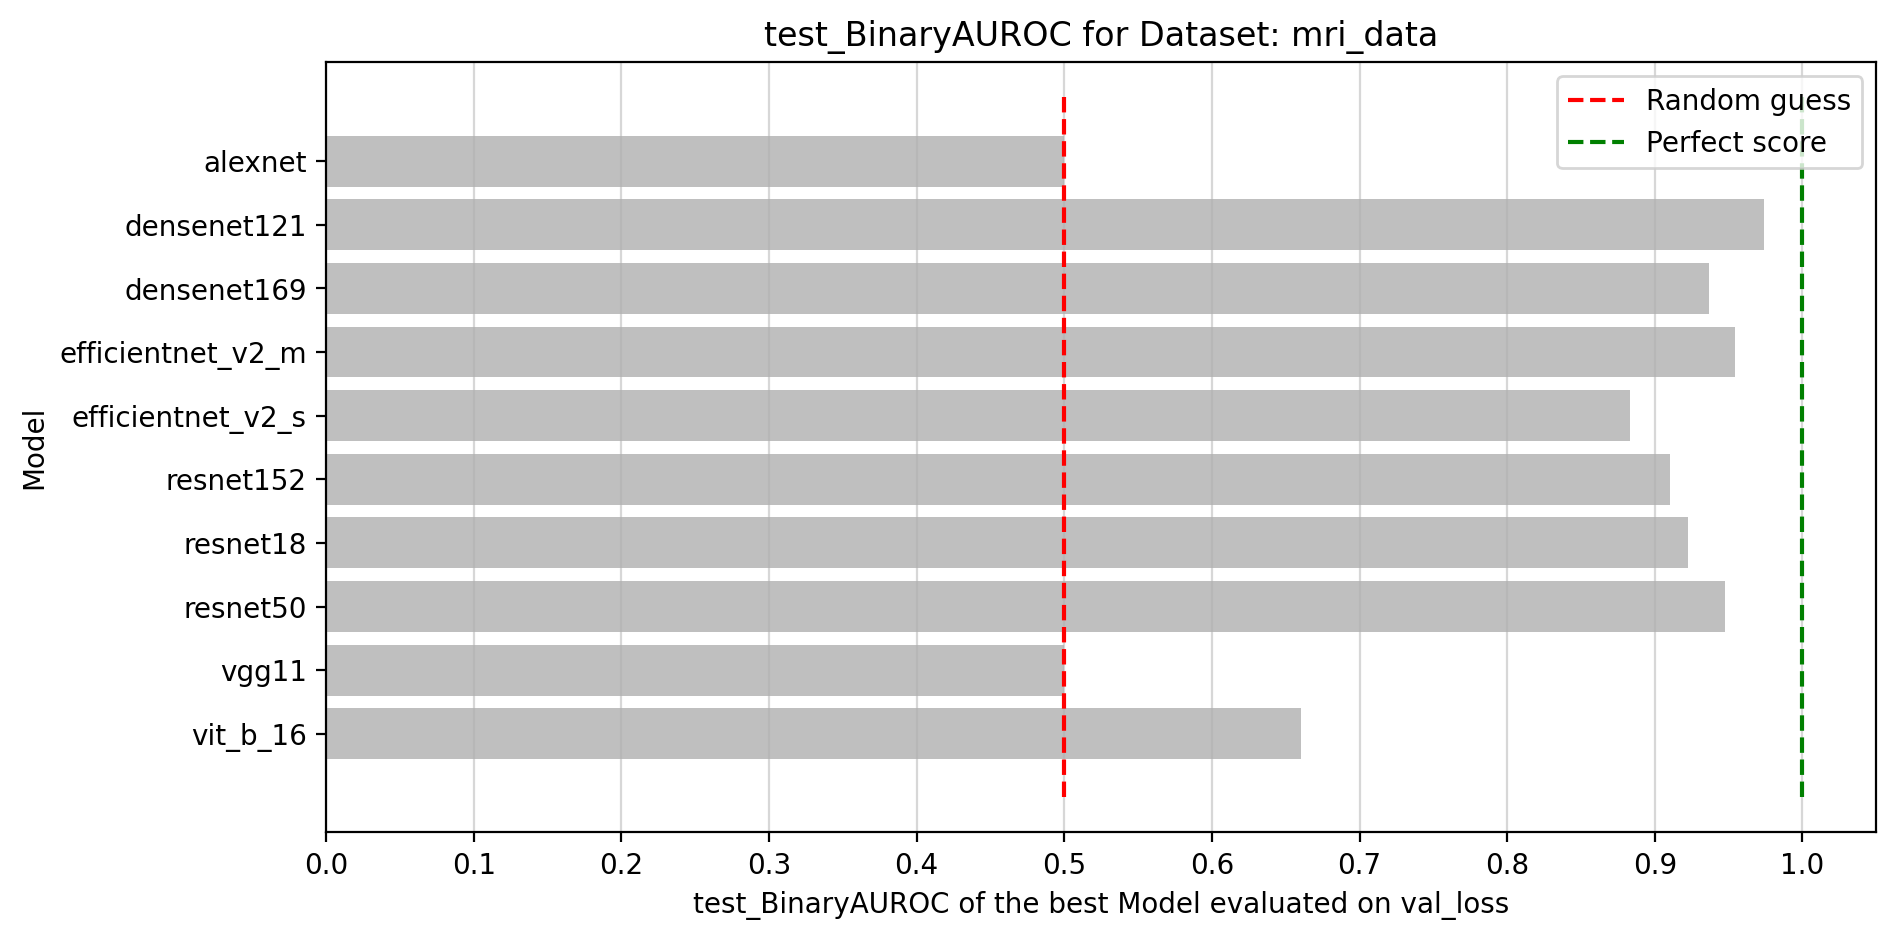
\includegraphics[height=0.5\linewidth]{01-images/05-resultate/test_binaryAUROC_MRI.png}
        \caption{AUROC-Testmetrik für den MRI-Datensatz}
    \end{subfigure}
    \caption{Die AUROC-Testmetriken der besten Modelle im Trainingslauf gemessen an der test\_loss-Metrik}
\end{figure}

Aufgrund der grossen Unterschiede zwischen dem Validierungs- und Testdatensatz erfolgt die Evaluation der Anfälligkeit der Modelle auf beiden Datensätzen.

\newpage

